\begin{figure}[t!]
    \centering
    \begin{subfigure}[b]{0.4\linewidth}
      \centering
      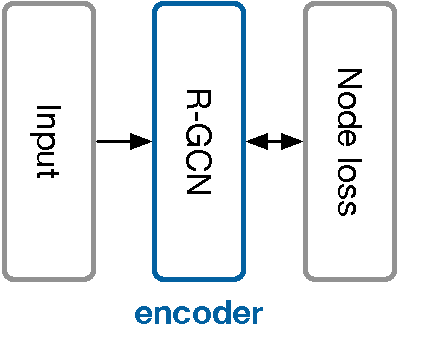
\includegraphics[width=0.90\linewidth, trim={0 0.2cm 0.6cm 0}, clip]{figures/entity-classification.pdf}
      \caption{Entity classification}        
      \label{fig:model-b}
    \end{subfigure}%
    ~\quad
    \begin{subfigure}[b]{0.49\linewidth}
        \centering
        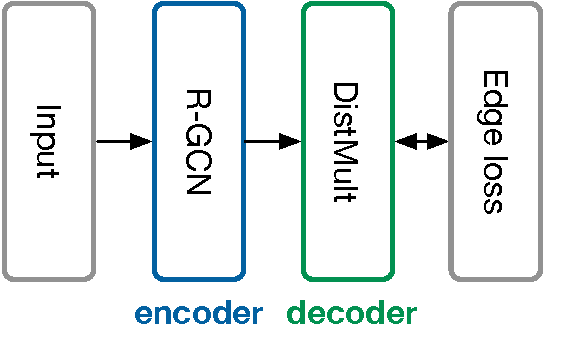
\includegraphics[width=\linewidth, trim={0 0.2cm 0.6cm 0}, clip]{figures/link-prediction.pdf}
        \caption{Link prediction}
        \label{fig:model-c}
    \end{subfigure}
    \caption{(a) Depiction of an R-GCN model for entity classification with a per-node loss function. (b) Link prediction model with an R-GCN encoder (interspersed with fully-connected/dense layers) and a DistMult decoder that takes pairs of hidden node representations and produces a score for every (potential) edge in the graph. The loss is evaluated per edge.}
\end{figure}

For (semi-)supervised classification of nodes (entities), we simply stack R-GCN layers of the form \eqref{eq:layer}, with a $\mathrm{softmax}(\cdot)$ activation (per node) on the output of the last layer. We minimize the following cross-entropy loss on all labeled nodes (while ignoring unlabeled nodes):
\begin{equation}
\mathcal{L}= -\sum_{i\in\mathcal{Y}}\sum_{k=1}^K t_{ik} \ln h_{ik}^{(L)}  \, ,
\label{eq:}
\end{equation} 
where $\mathcal{Y}$ is the set of node indices that have labels and $h_{ik}^{(L)}$ is the $k$-th entry of the network output for the $i$-th labeled node. $t_{ik}$ denotes its respective ground truth label. In practice, we train the model using (full-batch) gradient descent techniques. A schematic depiction of our entity classification model is given in Figure \ref{fig:model-b}.